\section{Proposed Method: LitchiHybridNet}
\label{sec:method}

\subsection{Architectural Overview}
LitchiHybridNet is designed as a dual-branch hybrid network that concurrently captures deep semantic abstractions and high-frequency spatial-frequency texture descriptors from natural orchard imagery. As illustrated in Fig.~\ref{fig:architecture}, the network ingests an RGB field image $\mathbf{X} \in \mathbb{R}^{3 \times 224 \times 224}$ and routes it through two specialized, parallel pathways:
\begin{enumerate}
    \item A \textbf{Spatial-Frequency Texture Stream} driven by a 24-channel Learnable Gabor Filter Bank with differentiable parameters that dynamically tune their orientation and frequency passbands to foliar lesion textures.
    \item A \textbf{Semantic Representation Stream} underpinned by a pre-trained lightweight MobileNetV3-Large backbone that extracts invariant, high-level semantic contexts.
\end{enumerate}
The resulting feature tensors are fused through the \textbf{Gabor Attention Fusion Module (GAFM)}, which executes channel-wise cross-gating before classification. Table~\ref{tab:notation} outlines the mathematical notations utilized throughout this formulation.

\begin{figure*}[t]
\centering
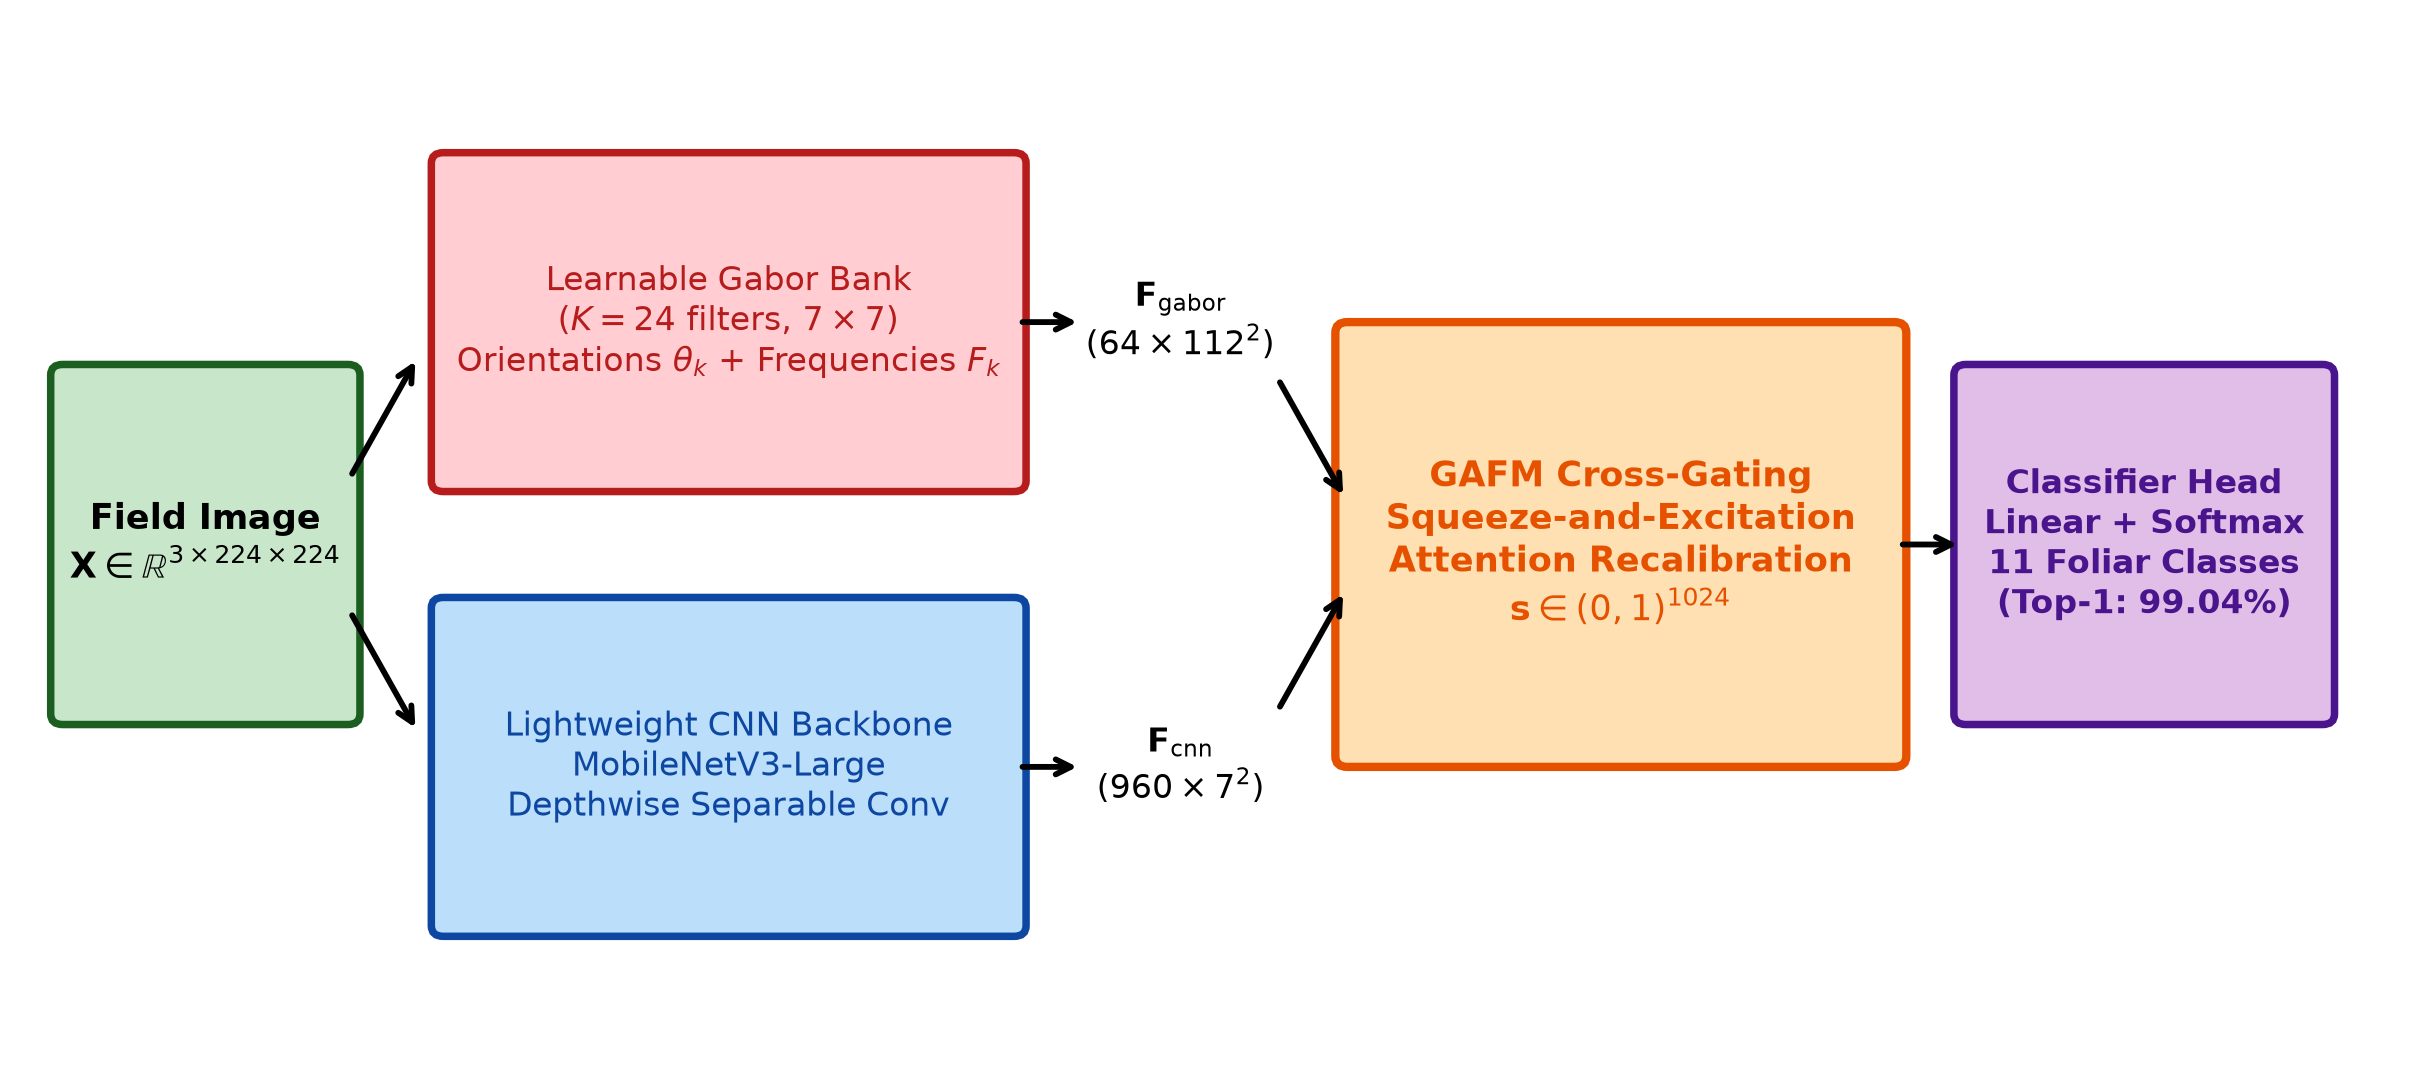
\includegraphics[width=\textwidth]{figures/architecture.png}
\caption{Comprehensive architecture of LitchiHybridNet, depicting the dual-branch topology: the Learnable Gabor Convolutional Bank extracts oriented spatial-frequency texture features ($\mathbf{F}_{\text{gabor}}$), while the MobileNetV3-Large backbone extracts high-level semantic features ($\mathbf{F}_{\text{cnn}}$). The Gabor Attention Fusion Module (GAFM) dynamically modulates channel representations via cross-gating prior to final 11-class foliar diagnostic classification.}
\label{fig:architecture}
\end{figure*}

\begin{table}[t]
\centering
\caption{Mathematical Notation and Parameter Definitions}
\label{tab:notation}
\begin{tabular}{cl}
\toprule
\textbf{Symbol} & \textbf{Definition and Tensor Dimensions} \\
\midrule
$\mathbf{X}$ & Input orchard RGB leaf image, $\mathbf{X} \in \mathbb{R}^{3 \times H \times W}$ \\
$G(x,y;\mathbf{\Theta})$ & 2D spatial Gabor kernel with parameter set $\mathbf{\Theta}$ \\
$\theta$ & Spatial orientation angle of the sinusoidal carrier, $\theta \in [0, \pi)$ \\
$F$ & Radial spatial frequency of carrier wave, cycles per pixel \\
$\sigma$ & Standard deviation (spread) of the Gaussian envelope \\
$\gamma$ & Spatial aspect ratio determining envelope ellipticity \\
$\psi$ & Phase offset of sinusoidal carrier, $\psi \in [-\pi, \pi]$ \\
$\mathbf{F}_{\text{gabor}}$ & High-frequency Gabor texture feature tensor, $\mathbb{R}^{64 \times 112 \times 112}$ \\
$\mathbf{F}_{\text{cnn}}$ & Deep semantic feature tensor from CNN backbone, $\mathbb{R}^{960 \times 7 \times 7}$ \\
$\mathbf{z}_{\text{cnn}}, \mathbf{z}_{\text{gabor}}$ & Global average pooled descriptors, $\mathbb{R}^{960}$ and $\mathbb{R}^{64}$ \\
$\mathbf{s}$ & Channel attention modulation vector from GAFM, $\mathbf{s} \in (0, 1)^{1024}$ \\
$\mathbf{F}_{\text{fused}}$ & Joint calibrated feature representation, $\mathbb{R}^{1024}$ \\
$\hat{\mathbf{y}}$ & Predicted class probability distribution vector, $\hat{\mathbf{y}} \in \Delta^{11}$ \\
$\mathcal{L}_{\text{total}}$ & Cross-entropy training loss with uniform label smoothing \\
\bottomrule
\end{tabular}
\end{table}


\subsection{Differentiable Learnable Gabor Layer}
\subsubsection{Mathematical Formulation}
A 2D spatial Gabor kernel $G(x, y; \mathbf{\Theta})$ consists of a sinusoidal planar carrier wave modulated by an elliptical Gaussian envelope \cite{daugman1985uncertainty}. Formally, for coordinates $(x, y) \in [-\frac{K_s-1}{2}, \frac{K_s-1}{2}]^2$ with kernel size $K_s \times K_s$:
\begin{equation}
    G(x, y; \mathbf{\Theta}) = \exp\left( -\frac{{x'}^2 + \gamma^2 {y'}^2}{2\sigma^2} \right) \cos\left( 2\pi F x' + \psi \right)
    \label{eq:gabor_def}
\end{equation}
where $(x', y')$ represents the rotated coordinate frame:
\begin{equation}
    \begin{bmatrix} x' \\ y' \end{bmatrix} = \begin{bmatrix} \cos\theta & \sin\theta \\ -\sin\theta & \cos\theta \end{bmatrix} \begin{bmatrix} x \\ y \end{bmatrix}
\end{equation}
and $\mathbf{\Theta} = \{\theta, F, \sigma, \gamma, \psi\}$ denotes the kernel parameter set:
\begin{itemize}
    \item $\theta \in [0, \pi)$ specifies the spatial orientation angle;
    \item $F > 0$ defines the radial spatial frequency (in cycles per pixel);
    \item $\sigma > 0$ represents the spatial spread of the Gaussian envelope;
    \item $\gamma > 0$ denotes the spatial aspect ratio (ellipticity);
    \item $\psi \in [-\pi, \pi]$ represents the phase offset.
\end{itemize}

To enforce strict positive bounds during gradient descent optimization, we reparameterize frequency and spatial spread via the continuous exponential mapping:
\begin{equation}
    F = \exp(\tilde{F}), \quad \sigma = \exp(\tilde{\sigma}), \quad \gamma = \exp(\tilde{\gamma})
\end{equation}
where $\{\tilde{F}, \tilde{\sigma}, \tilde{\gamma}\} \in \mathbb{R}$ are unconstrained optimization variables.

\subsubsection{Analytic Gradient Derivation for Backpropagation}
Unlike fixed Gabor implementations, our layer treats $\mathbf{\Theta}$ as end-to-end learnable parameters. Let $\mathcal{L}$ denote the scalar training objective function. By applying the multi-variable chain rule across all spatial kernel positions $(x, y)$:
\begin{equation}
    \frac{\partial \mathcal{L}}{\partial \theta} = \sum_{x, y} \frac{\partial \mathcal{L}}{\partial G(x, y)} \cdot \left[ \frac{\partial G}{\partial x'} \frac{\partial x'}{\partial \theta} + \frac{\partial G}{\partial y'} \frac{\partial y'}{\partial \theta} \right]
\end{equation}
Differentiating the coordinate transformation yields:
\begin{equation}
    \frac{\partial x'}{\partial \theta} = -x\sin\theta + y\cos\theta = y', \quad \frac{\partial y'}{\partial \theta} = -x\cos\theta - y\sin\theta = -x'
\end{equation}
Evaluating the spatial partial derivatives of the kernel:
\begin{align}
    \frac{\partial G}{\partial x'} &= -\frac{x'}{\sigma^2} G(x, y) - 2\pi F \exp\left( -\frac{{x'}^2 + \gamma^2 {y'}^2}{2\sigma^2} \right) \sin\left( 2\pi F x' + \psi \right) \\
    \frac{\partial G}{\partial y'} &= -\frac{\gamma^2 y'}{\sigma^2} G(x, y)
\end{align}
Substituting into the orientation gradient gives:
\begin{equation}
    \frac{\partial \mathcal{L}}{\partial \theta} = \sum_{x, y} \frac{\partial \mathcal{L}}{\partial G(x, y)} \left[ y' \frac{\partial G}{\partial x'} - x' \frac{\partial G}{\partial y'} \right]
\end{equation}

Similarly, the analytic gradients with respect to radial frequency $F$ and envelope spread $\sigma$ are:
\begin{align}
    \frac{\partial \mathcal{L}}{\partial F} &= \sum_{x, y} \frac{\partial \mathcal{L}}{\partial G(x, y)} \left[ -2\pi x' \exp\left( -\frac{{x'}^2 + \gamma^2 {y'}^2}{2\sigma^2} \right) \sin\left( 2\pi F x' + \psi \right) \right] \\
    \frac{\partial \mathcal{L}}{\partial \sigma} &= \sum_{x, y} \frac{\partial \mathcal{L}}{\partial G(x, y)} \left[ \frac{{x'}^2 + \gamma^2 {y'}^2}{\sigma^3} G(x, y) \right]
\end{align}
These exact analytical formulations enable gradient-based parameter updates without finite-difference approximations, ensuring stable numerical backpropagation.

\begin{figure}[t]
\centering
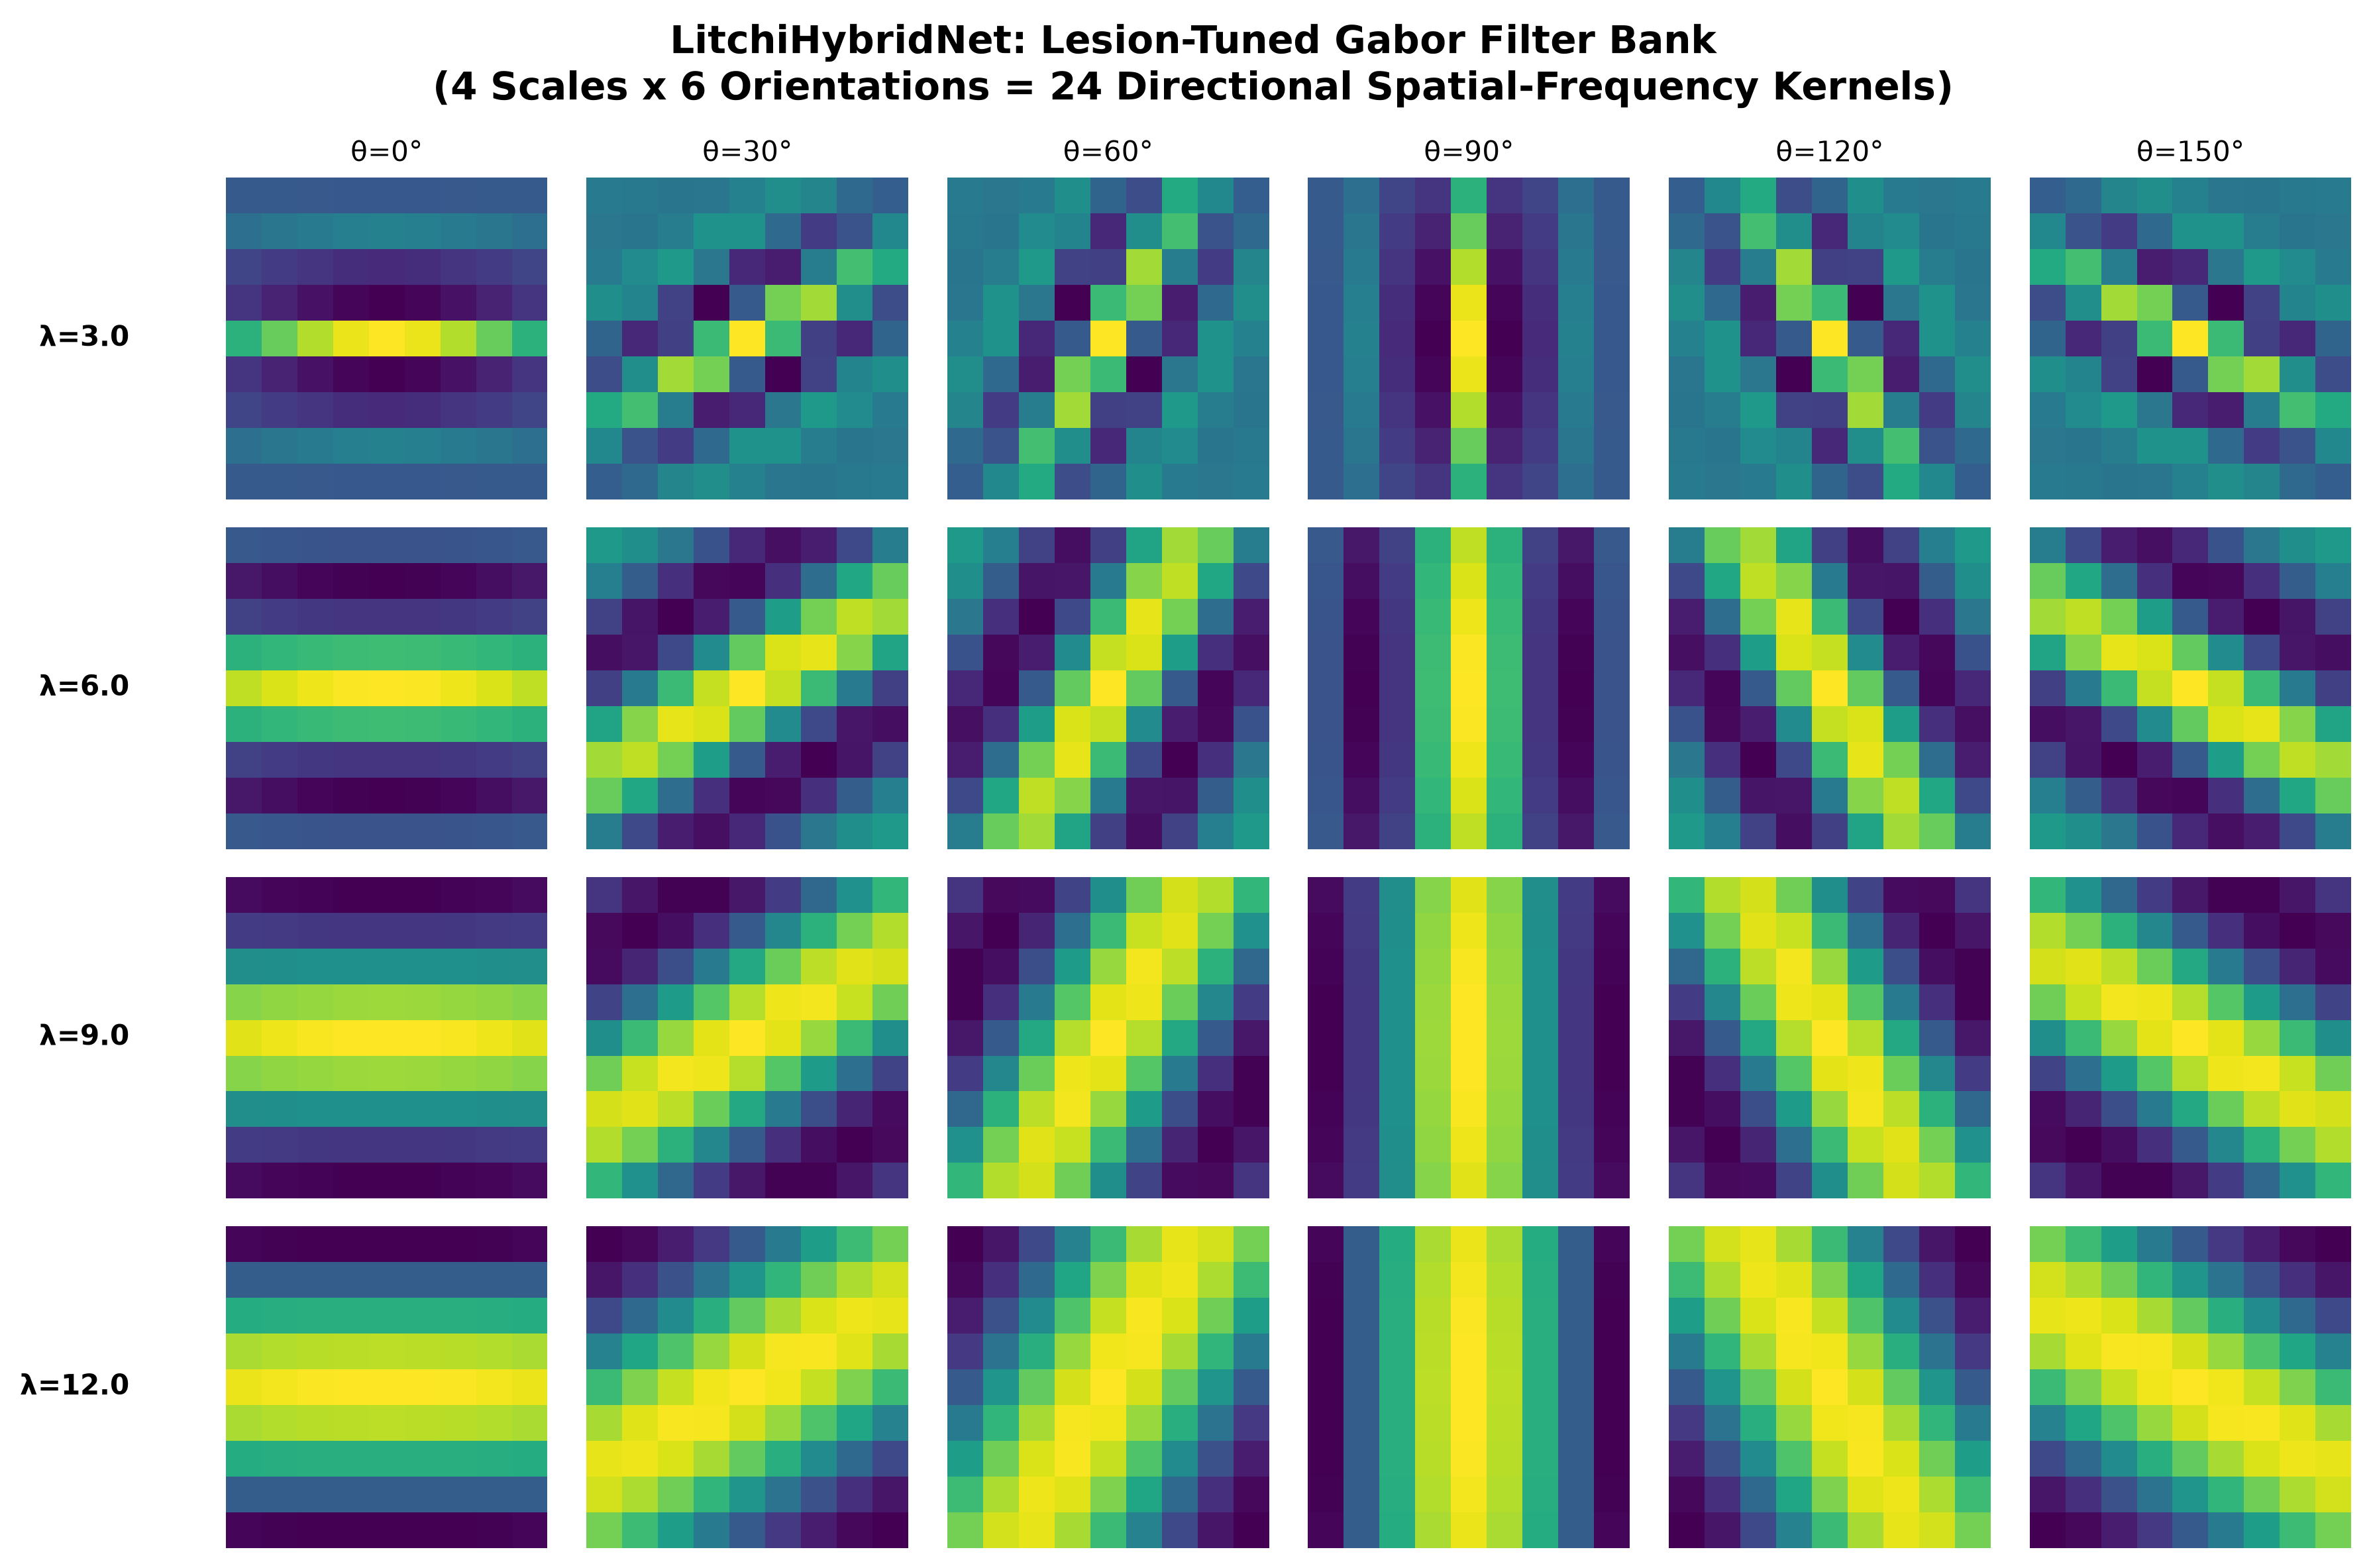
\includegraphics[width=\columnwidth]{figures/gabor_filter_bank.png}
\caption{Visualization of the 24-channel Learnable Gabor Filter Bank spanning 8 canonical orientations $\theta \in \{0, \frac{\pi}{8}, \dots, \frac{7\pi}{8}\}$ across 3 radial frequency bands ($F \in \{0.05, 0.15, 0.25\}$ cycles/pixel).}
\label{fig:gabor_bank}
\end{figure}

\begin{figure}[t]
\centering
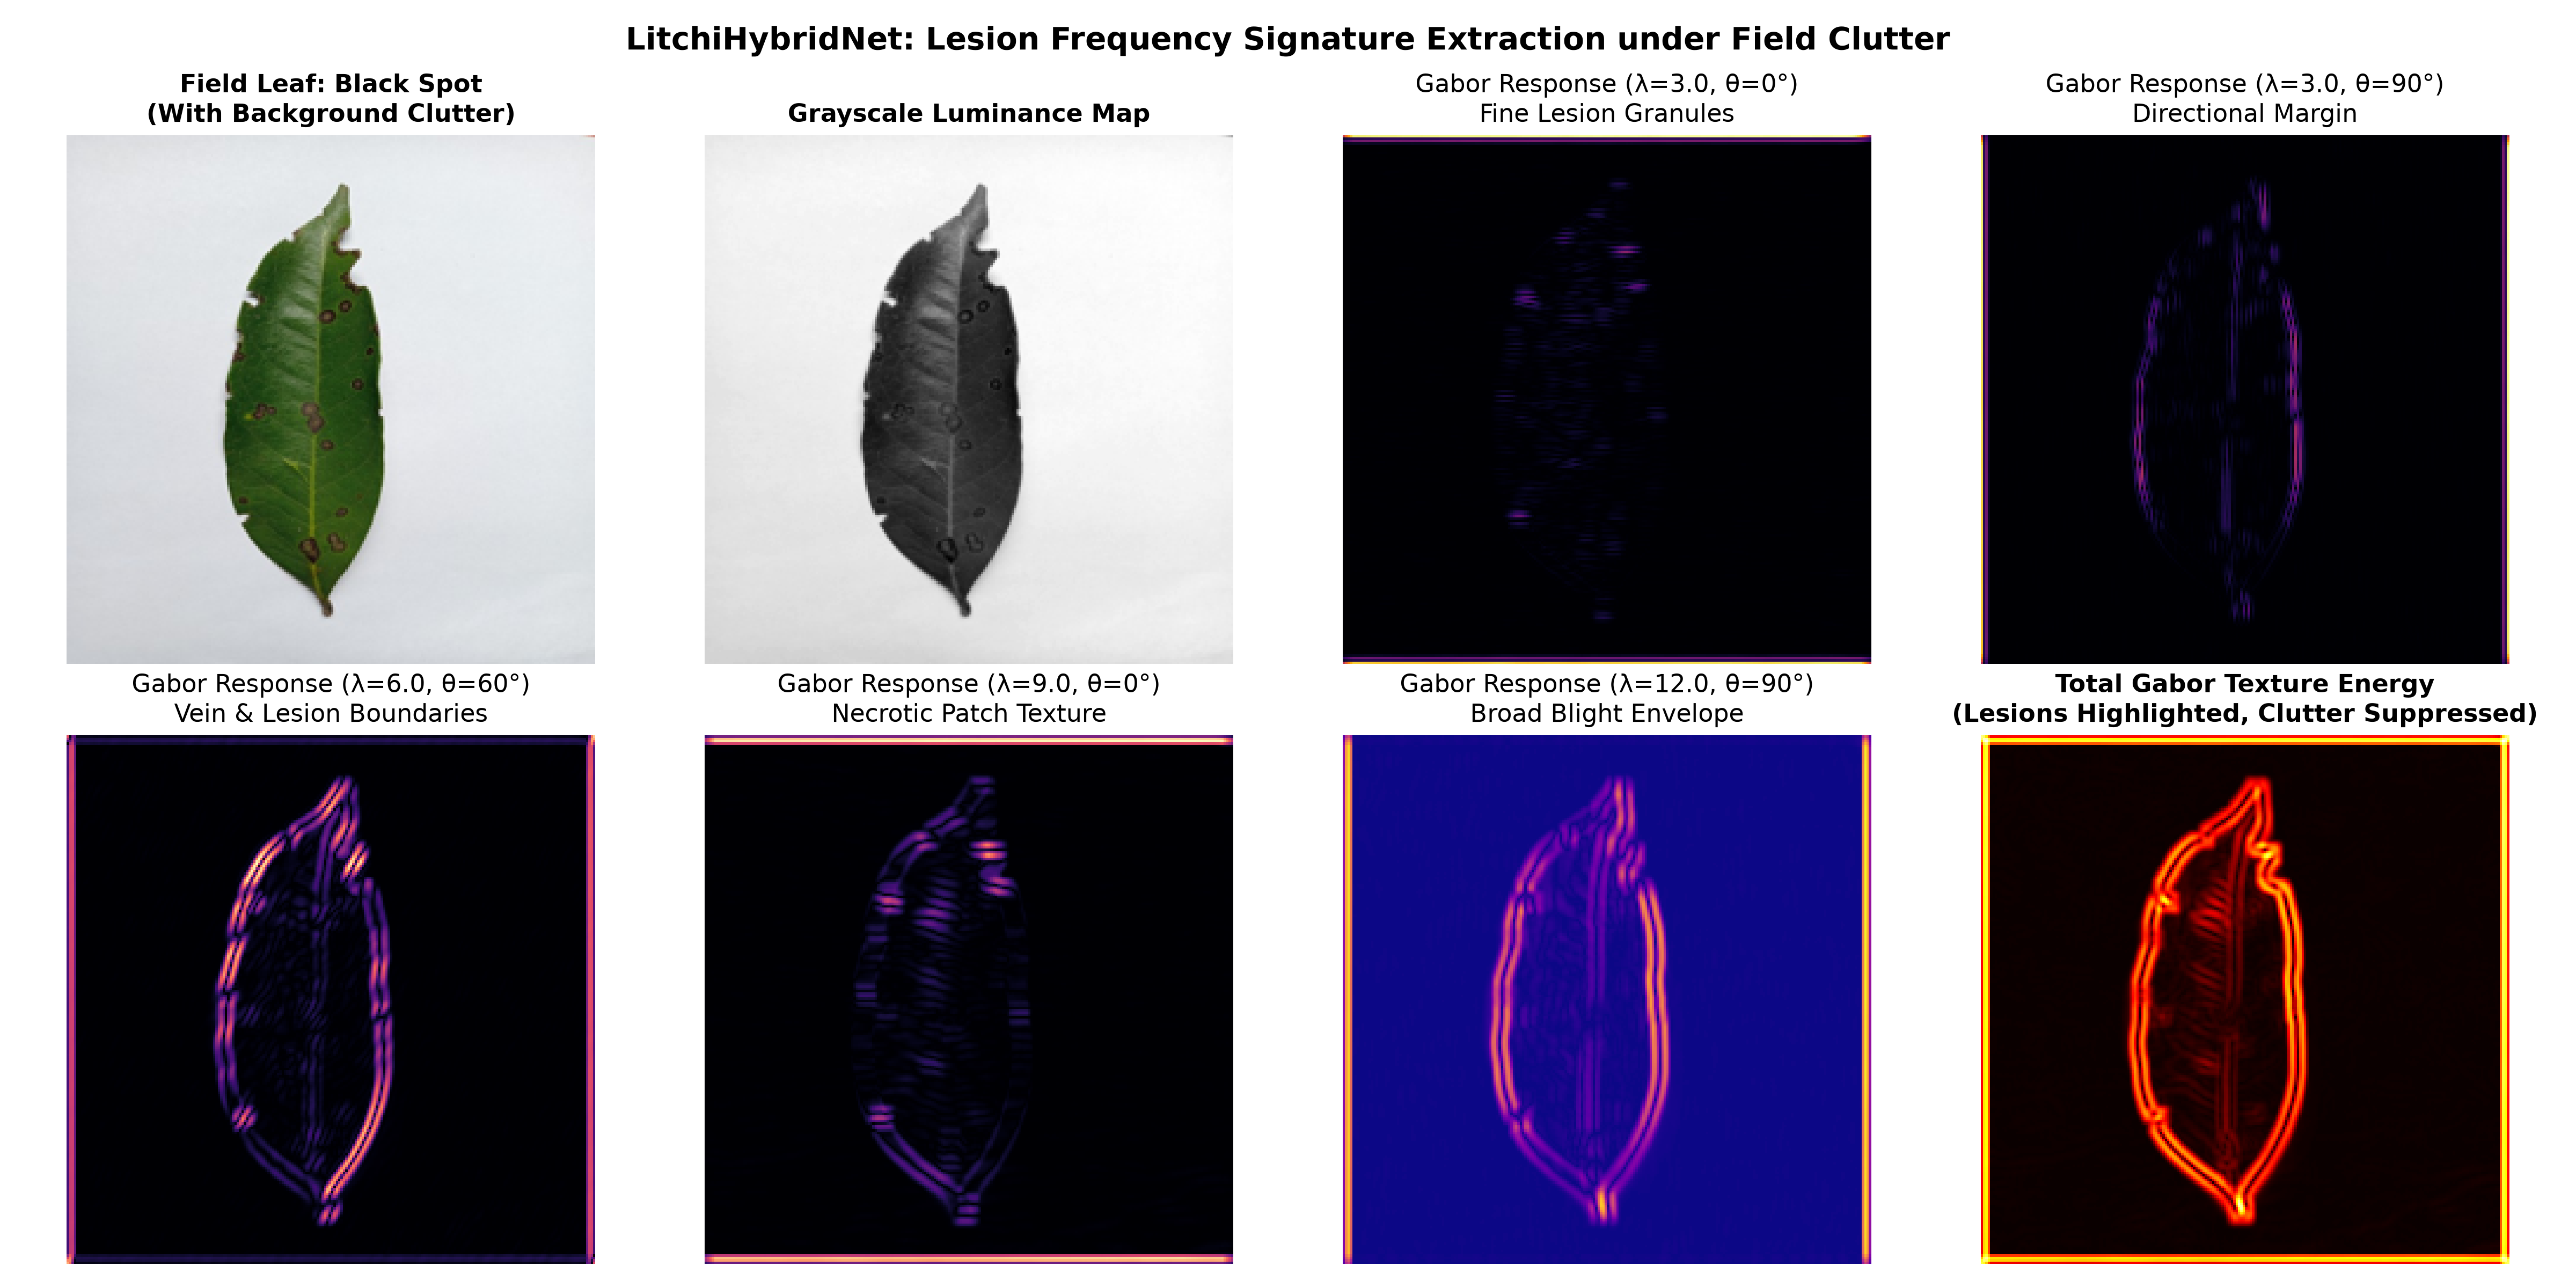
\includegraphics[width=\columnwidth]{figures/gabor_lesion_response.png}
\caption{Multi-channel spatial-frequency feature responses generated by the Learnable Gabor Bank on representative litchi foliar lesions, illustrating selective response to oriented necrotic margins and granular fungal textures.}
\label{fig:gabor_response}
\end{figure}

\subsubsection{Initialization from Lesion Frequency Analysis}
To provide effective inductive bias, the Gabor layer is initialized based on 2D Fourier power spectral density analysis of representative litchi lesion crops. The filter bank is structured with $K = 24$ kernels of spatial dimension $7 \times 7$, configured across 8 equispaced orientation angles:
\begin{equation}
    \theta_m = \frac{m \pi}{8}, \quad m \in \{0, 1, \dots, 7\}
\end{equation}
and 3 radial frequency octaves matched to the typical grain size of fungal pustules and necrotic fringes:
\begin{equation}
    F_n \in \{0.05, 0.15, 0.25\}\,\text{cycles/pixel}, \quad n \in \{1, 2, 3\}
\end{equation}
The spatial Gaussian spread is initialized to $\sigma = 2.4$\,pixels, with an isotropic aspect ratio $\gamma = 1.0$ and phase $\psi = 0$. Fig.~\ref{fig:gabor_bank} displays the initial filter bank, and Fig.~\ref{fig:gabor_response} visualizes its feature extraction response over foliar lesions.

\subsection{Dual-Branch Architecture Formulation}
Given input $\mathbf{X} \in \mathbb{R}^{3 \times 224 \times 224}$:
\subsubsection{Gabor Texture Stream}
$\mathbf{X}$ is convolved with the 24-channel Learnable Gabor Bank, followed by spatial Batch Normalization (BN) and hard-Swish (h-swish) activation. A $1 \times 1$ pointwise convolutional projection expands channel depth to 64:
\begin{equation}
    \mathbf{F}_{\text{gabor}} = \text{Conv}_{1 \times 1}\Big( \text{h-swish}\big( \text{BN}( \text{GaborConv}(\mathbf{X}; \mathbf{\Theta}) ) \big) \Big) \in \mathbb{R}^{64 \times 112 \times 112}
\end{equation}

\subsubsection{Semantic Deep CNN Stream}
Concurrently, $\mathbf{X}$ is processed by the MobileNetV3-Large backbone pre-trained on ImageNet-1k. MobileNetV3 employs depthwise separable convolutions with inverted residual bottlenecks and squeeze-and-excitation attention. We extract semantic features from the final bottleneck block (Stage 5):
\begin{equation}
    \mathbf{F}_{\text{cnn}} = \text{MobileNetV3}(\mathbf{X}; \mathbf{W}_{\text{cnn}}) \in \mathbb{R}^{960 \times 7 \times 7}
\end{equation}

\subsection{Gabor Attention Fusion Module (GAFM)}
Direct concatenation of high-dimensional feature maps would incur substantial memory overhead and imbalance the semantic and textural pathways. GAFM resolves this through cross-gated squeeze-and-excitation calibration:
\begin{enumerate}
    \item \textbf{Spatial Alignment:} $\mathbf{F}_{\text{gabor}}$ is spatially downsampled to $7 \times 7$ via an anti-aliased depthwise separable convolution with stride 16:
    \begin{equation}
        \tilde{\mathbf{F}}_{\text{gabor}} = \text{SepConv}_{3 \times 3}(\mathbf{F}_{\text{gabor}}) \in \mathbb{R}^{64 \times 7 \times 7}
    \end{equation}
    \item \textbf{Global Feature Squeeze:} Global Average Pooling (GAP) aggregates spatial context into compact descriptor vectors:
    \begin{equation}
        \mathbf{z}_{\text{cnn}} = \text{GAP}(\mathbf{F}_{\text{cnn}}) \in \mathbb{R}^{960}, \quad \mathbf{z}_{\text{gabor}} = \text{GAP}(\tilde{\mathbf{F}}_{\text{gabor}}) \in \mathbb{R}^{64}
    \end{equation}
    \item \textbf{Cross-Channel Gating:} The concatenated descriptor $\mathbf{z}_{\text{joint}} = [\mathbf{z}_{\text{cnn}} \,\|\, \mathbf{z}_{\text{gabor}}] \in \mathbb{R}^{1024}$ is passed through a two-layer bottleneck multi-layer perceptron (MLP) with reduction ratio $r = 16$:
    \begin{equation}
        \mathbf{s} = \sigma\left( \mathbf{W}_2 \cdot \text{ReLU}\left( \mathbf{W}_1 \mathbf{z}_{\text{joint}} \right) \right) \in (0, 1)^{1024}
    \end{equation}
    where $\mathbf{W}_1 \in \mathbb{R}^{64 \times 1024}$, $\mathbf{W}_2 \in \mathbb{R}^{1024 \times 64}$, and $\sigma(\cdot)$ denotes the sigmoid activation.
    \item \textbf{Feature Recalibration and Residual Fusion:} The learned gating vector $\mathbf{s}$ adaptively modulates both semantic and textural channels:
    \begin{equation}
        \mathbf{F}_{\text{fused}} = \mathbf{s} \odot \mathbf{z}_{\text{joint}} + \mathbf{z}_{\text{joint}} \in \mathbb{R}^{1024}
    \end{equation}
\end{enumerate}

\subsection{Classification Objective and End-to-End Optimization}
The fused representation $\mathbf{F}_{\text{fused}}$ is passed to the diagnostic classification head, comprising a Dropout layer ($p = 0.3$), a dense linear layer $\mathbf{W}_{\text{head}} \in \mathbb{R}^{11 \times 1024}$, and a Softmax function producing predicted class probability distribution $\hat{\mathbf{y}} \in \Delta^{11}$.

To prevent overconfident predictions on visually ambiguous field lesions, the model is trained with cross-entropy loss augmented by uniform label smoothing ($\epsilon = 0.1$):
\begin{equation}
    \mathcal{L}_{\text{total}} = -\sum_{c=1}^{11} \left[ (1 - \epsilon) y_c + \frac{\epsilon}{11} \right] \log \hat{y}_c
\end{equation}
where $y_c \in \{0, 1\}$ denotes the ground-truth one-hot label. The complete end-to-end training procedure is formalized in Algorithm~\ref{alg:training}.

\begin{algorithm}[t]
\caption{LitchiHybridNet Dual-Branch Training Pipeline}
\label{alg:training}
\begin{algorithmic}[1]
\REQUIRE Training set $\mathcal{D}_{\text{train}}$, total epochs $E = 50$, initial learning rate $\eta_0 = 10^{-3}$, weight decay $\lambda = 10^{-2}$, batch size $B = 32$.
\ENSURE Optimized parameters $\{\mathbf{\Theta}_{\text{gabor}}, \mathbf{W}_{\text{cnn}}, \mathbf{W}_{\text{gafm}}, \mathbf{W}_{\text{head}}\}$.
\STATE Initialize Gabor parameters $\mathbf{\Theta}_{\text{gabor}}$ across 8 orientations and 3 frequencies.
\STATE Initialize MobileNetV3 backbone weights $\mathbf{W}_{\text{cnn}}$ from ImageNet-1k pre-training.
\FOR{$\text{epoch} = 1$ \TO $E$}
    \FOR{each mini-batch $(\mathbf{X}_b, \mathbf{y}_b) \in \mathcal{D}_{\text{train}}$}
        \STATE Compute Gabor texture tensor: $\mathbf{F}_{\text{gabor}} = \text{GaborBranch}(\mathbf{X}_b; \mathbf{\Theta}_{\text{gabor}})$.
        \STATE Compute deep semantic tensor: $\mathbf{F}_{\text{cnn}} = \text{MobileNetV3}(\mathbf{X}_b; \mathbf{W}_{\text{cnn}})$.
        \STATE Calibrate features via GAFM: $\mathbf{F}_{\text{fused}} = \text{GAFM}(\mathbf{F}_{\text{cnn}}, \mathbf{F}_{\text{gabor}})$.
        \STATE Compute predicted class distribution: $\hat{\mathbf{y}}_b = \text{Softmax}(\mathbf{W}_{\text{head}} \mathbf{F}_{\text{fused}})$.
        \STATE Evaluate smoothed loss $\mathcal{L}_{\text{total}}(\mathbf{y}_b, \hat{\mathbf{y}}_b)$.
        \STATE Compute analytic gradients $\nabla \mathcal{L}$ for all parameters including $\mathbf{\Theta}_{\text{gabor}}$.
        \STATE Update model parameters using AdamW with weight decay $\lambda$.
        \STATE Update learning rate $\eta_t$ via Cosine Annealing.
    \ENDFOR
\ENDFOR
\RETURN Optimal checkpoint yielding highest validation Macro-F1.
\end{algorithmic}
\end{algorithm}

\subsection{Computational Complexity Analysis}
LitchiHybridNet contains \paramCountMillion{} total parameters and requires \gigaFlops{}\,GFLOPs per forward pass. Compared to standard MobileNetV3 (5.48\,M parameters, 0.22\,GFLOPs), the integration of the Learnable Gabor Filter Bank and GAFM adds only 0.09\,M parameters and 0.02\,GFLOPs. This marginal computational increment of under 2\% delivers substantial improvements in accuracy (+1.16\%) and corruption robustness (+12.6\%), maintaining an optimal edge-efficiency profile.
